\documentclass[convert={outext=.png}]{standalone}
\usepackage{tikz}

% Compile with: lulatex -shell-escape vrft_block_diagram_standalone.tex

\tikzset{
	block/.style  = {draw, fill=white, rectangle, minimum height=3em, minimum width=3em, node distance = 2cm},
	sum/.style    = {draw, fill=white, circle, node distance=1cm},
	input/.style  = {coordinate},
	output/.style = {coordinate},
	hidden/.style  = {coordinate},
}

\begin{document}
	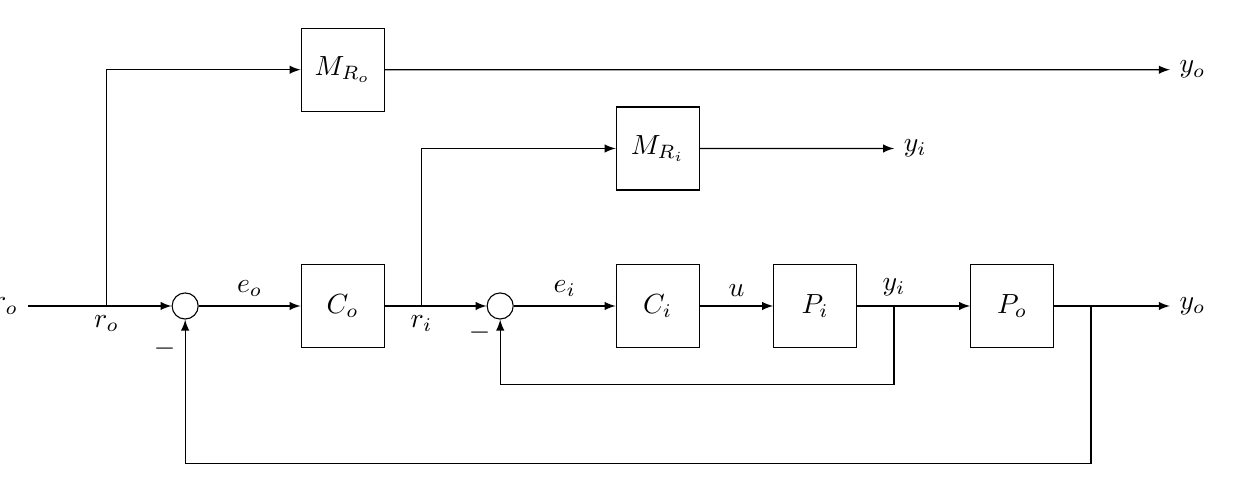
\begin{tikzpicture}[auto, trim left, scale=0.1, >=latex]
	% Draw the main control loop nodes
	\draw
	node[input] (input) {}
	node[hidden, right of = input        ] (oinputfork) {}
	node[sum   , right of = oinputfork   ] (osum) {}
	node[block , right of = osum         ] (ocontroller) {$C_o$}
	node[hidden, right of = ocontroller  ] (iinputfork) {}
	node[sum   , right of = iinputfork   ] (isum) {}
	node[block , right of = isum         ] (icontroller) {$C_i$}
	node[block , right of = icontroller  ] (iplant) {$P_i$}
	node[hidden, right of = iplant       ] (ioutputfork) {}
	node[block , right of = ioutputfork  , node distance = 1.5cm] (oplant) {$P_o$}
	node[hidden, right of = oplant       ] (ooutputfork) {}
	node[output, right of = ooutputfork  ] (output) {}
	node[hidden, below of = iplant       ] (iretroaction) {}
	node[hidden, below of = iplant       ] (iretroaction) {}
	node[hidden, below of = iretroaction ] (oretroaction) {};
	
	% Draw the reference model nodes
	\draw
	node[block , above of = icontroller] (irefmodel) {$M_{R_i}$}
	node[coordinate] at (irefmodel -| ioutputfork) (irefoutput) {};
	
	\draw
	node[hidden, above of = irefmodel] (orefheight) {}
	node[block] at (orefheight -| ocontroller) (orefmodel) {$M_{R_o}$}
	node[coordinate] at (orefmodel -| output) (orefoutput) {};
	
	% Connect everything together
	\draw[->] node[left] {$r_o$} (input) -- (oinputfork)  -- (osum);
	\draw[->] (osum) -- (ocontroller) node[midway] {$e_o$};
	\draw[->] (ocontroller) -- (iinputfork) -- (isum);
	\draw[->] (isum) -- (icontroller) node[midway] {$e_i$};
	\draw[->] (icontroller) -- (iplant) node[midway] {$u$};
	\draw[->] (iplant) -- (ioutputfork) node[above] {$y_i$} -- (oplant) ;
	\draw[->] (oplant) -- (ooutputfork) -- (output) node[right] {$y_o$};
	
	% Draw retroactions
	\draw[->] (ioutputfork) |- (iretroaction) -| (isum) node[pos=0.9] {$-$};
	\draw[->] (ooutputfork) |- (oretroaction) -| (osum) node[pos=0.9] {$-$};
	
	% Draw reference models
	\draw[->] (iinputfork) node[below] {$r_i$} |- (irefmodel);
	\draw[->] (irefmodel) -- (irefoutput) node[right] {$y_i$};
	
	\draw[->] (oinputfork) node[below] {$r_o$} |- (orefmodel);
	\draw[->] (orefmodel) -- (orefoutput) node[right] {$y_o$};
	
	\end{tikzpicture}
	
\end{document}